% %-------------------------------------------------------------------------------
%	PAQUETES Y OTRAS CONFIGURACIONES DEL DOCUMENTO
%-------------------------------------------------------------------------------

\documentclass[twoside]{book}

\usepackage[spanish]{babel}
\usepackage[utf8]{inputenc}
%\usepackage[latin1]{inputenc}
\usepackage{amsmath}

%\usepackage{lipsum} % Package to generate dummy text throughout this template

\usepackage[sc]{mathpazo} % Use the Palatino font
\usepackage[T1]{fontenc} % Use 8-bit encoding that has 256 glyphs
\linespread{1.05} % Line spacing - Palatino needs more space between lines
\usepackage{microtype} % Slightly tweak font spacing for aesthetics

\usepackage[hmarginratio=1:1,top=32mm,columnsep=20pt]{geometry} % Document margins
\usepackage{multicol} % Used for the two-column layout of the document
\usepackage[hang, small,labelfont=bf,up,textfont=it,up]{caption} % Custom captions under/above floats in tables or figures
\usepackage{booktabs} % Horizontal rules in tables
\usepackage{float} % Required for tables and figures in the multi-column environment - they need to be placed in specific locations with the [H] (e.g. \begin{table}[H])
\usepackage{hyperref} % For hyperlinks in the PDF

\usepackage{lettrine} % The lettrine is the first enlarged letter at the beginning of the text
\usepackage{paralist} % Used for the compactitem environment which makes bullet points with less space between them

%\usepackage{abstract} % Allows abstract customization
%\renewcommand{\abstractnamefont}{\normalfont\bfseries} % Set the "Abstract" text to bold
%\renewcommand{\abstracttextfont}{\normalfont\small\itshape} % Set the abstract itself to small italic text

\usepackage{titlesec} % Allows customization of titles
\renewcommand\thesection{\Roman{section}} % Roman numerals for the sections
\renewcommand\thesubsection{\Roman{subsection}} % Roman numerals for subsections
\titleformat{\section}[block]{\large\scshape\centering}{\thesection.}{1em}{} % Change the look of the section titles
\titleformat{\subsection}[block]{\large}{\thesubsection.}{1em}{} % Change the look of the section titles

\usepackage{fancyhdr} % Headers and footers
\pagestyle{fancy} % All pages have headers and footers
\fancyhead{} % Blank out the default header
\fancyfoot{} % Blank out the default footer
\fancyhead[C]{Modelado y Simulación $\bullet$ 17 de Diciembre de 2014 $\bullet$ Proyectos} % Custom header text
\fancyfoot[RO,LE]{\thepage} % Custom footer text

\newtheorem{defi}{Definición}
\newtheorem{teo}{Teorema}
\newtheorem{ley}{Ley}
\newtheorem{prop}{Proposición}

\usepackage{graphicx}

%-------------------------------------------------------------------------------
%	FIN DE LAS CONFIGURACIONES
%-------------------------------------------------------------------------------

%
% \title{Tensegrity and Mechanical Stability of Vegetal Tissue}
% \author{Roberto Cadena Vega \\ Christian Alberto Villegas Elizalde}
%
% \begin{document}
% 	\maketitle
% 	\tableofcontents
%------------------------------------
%         Begin document
%------------------------------------
   	\section{Introduction and Motivation}
		\subsection{Introduction}
    %\input{Introduccion.tex}



\subsection{What is a Tensegrity?}
    %\input{whatisatensegrity.tex}



\subsection{Benefits of Tensegrity Design}
    %\input{TheBenefitsofTensegrity.tex}


%----------------------------------------
	\section{Tensegrity Structures in Biological Systems}
		
\subsection{Biochemistry and tensegrity structures}

    Cellular biochemistry plays out in a world of structural complexity that is nothing like the controlled solution of a test tube. Rather than being filled with a liquid ‘protoplasm’ as imagined a century ago, eukaryotic cells contain an intricate molecular framework, the cytoskeleton, composed of interconnected microfilaments, microtubules and intermediate filaments within their viscous cytosol (Heuser and Kirschner, 1980; Fey et al., 1984). Cytoskeletal filaments both generate and resist mechanical loads, and they are largely responsible for the cell’s ability to resist shape distortion. These scaffolds also function as tracks for the movement of organelles, and they orient many of the enzymes and substrates involved in biochemical reactions that mediate critical cellular functions (Ingber, 1993a; Janmey, 1998). Moreover, cells respond to mechanical forces and to changes in cell shape or cytoskeletal structure by altering these same chemical activities (reviewed in Chicurel et al., 1998).

\subsection{Celular Tensegrity}

    Tensegrity is a principle building that was first described by architect R. Buckminster Fuller (Fuller, 1961) and the first visualized by sculptor Kenneth Snelson (Snelson, 1996). Fuller defined tensegrity systems and structures that stabilize its shape by the DC voltage or \emph{tensional integrity}.

    According to the most general definition of Fuller, tensegrity includes two broad structural classes - prestressed and Geodetic - that would both stop acting as a single entity or to maintain its shape stability when stressed mechanically without streaming tension forces (Fuller , 1961; Fuller, 1979; Ingber, 1998; Chen and Ingber, 1999). The first hold joints in position as a result of \emph{preload}  (pre-existing tensile stress or isometric tension) within the structure.

    Our bodies are a familiar example of a prestressed tensegrity structure: our bones act as props to resist the pull of muscles traction, tendons and ligaments, and shape stability (stiffness) of our body varies depending on the pitch (preload) in muscles. Examples of geodesic tensegrity structures include Fuller's geodesic domes, buckminsterfullerenes carbon based (Bucky balls), and the tetrahedral space frames, which are popular with NASA because they maintain stability in the absence of gravity and, therefore uncompressed carry on.

\subsection{¿Does cells utilize tensegrity architecture?}

    Biophysical studies with microfilaments and microtubules isolated revealed that the former are better in tensile strength, while blanks with microtubules mostly second moment of inertia are much more effective to resist compression (Mizushima-Sugano et al., 1983) . Because of its greater stiffness (persistence length), microtubules are rigid and straight when in solution and even expel extensions long membrane when enclosed in liposomes (Hotani and Miyamoto, 1990), while isolates microfilaments and intermediate filaments are bent or very tangled, respectively (Janmey et al., 1991; Mackintosh and Janmey, 1995).

    Studies of both cultured cells and whole tissues indicate that the stability of shape of the cell depends on a balance between microtubules and microfilaments contractile opposite.

\subsection{¿Does the citoskeleton behaves as a discrete mechanical network?}

    Mechanical established models developed by cell biologists and engineers assume that dense cortical microfilaments network that is directly below the cell membrane is the support element in the primary load cell (Albrecht-Buehler, 1987; Evans and Yeung, 1989; Dong et al., 1991; Fung and Liu, 1993; Schmid-Schönbein et al, 1995) .. These models predict that externally applied stresses are transmitted into the cell equally at all points in the cell surface and are borne by the cell cortex.

    In contrast, tensegrity model predicts that mechanical loads are supported by discrete molecular networks that span the cell surface and extend through the cytoplasm. More specifically, the transmembrane anchor extracellular molecules that physically couple (eg ECM molecules or cell-cell adhesion) to the internal cytoskeleton network must provide preferred routes for transferring mechanical stress within the cell, while other receptors transmembrane locally dissipate stress and thus stop transmitting the same signals. If the cell is a prestressed tensegrity structure, then a local effort can lead to global structural rearrangements, even remotely. This is because the discrete structural elements within the network change orientation load bearing and relative spacing to one another until a new equilibrium configuration is reached. Therefore, tensegrity model differs from conventional cell in which the application of local stress on the cell surface can result in the directed deformation of structures, both locally and deep within the cell, depending on the molecular connectivity through the membrane surface and through the viscous cytosol.

    Ning Wang, Donald E. Ingber set to discriminate between these models conflicting by developing a method called cytometry micromanipulation magnetic torque control where the mechanical stresses are applied directly to cell surface receptors by applying torque (shear stress) for receptor bound to magnetic microbeads (~ 1 to 10 microns in diameter) (Wang et al., 1993; Wang and Ingber, 1994; Wang and Ingber, 1995). In separate studies, magnetic tweezers (Bausch et al, 1998; Alenghat .. et al, 2000) were developed and used to apply stress to the cells of linear voltage, and optical tweezers are used to manipulate non-magnetic beads that were bound cell similar to -Surface receptors (Schmidt et al, 1993; Choquet et al .., 1997) manner.
    Mathematical formulation of the theory of tensegrity

    The theory of cellular tensegrity model was initially an intuitive and prestressed tensegrity structures built of sticks and elastic cords are used to display the (Ingber and Jamieson, 1985; Ingber, 1993b; Wang et al., 1993) concept.

    Another model, composed of multiple tensionally straws together by elastic cord, kinematically transformed into three-dimensional shapes that closely resemble the structures observed in actin stress fibers geodomes and living cells by light and electron microscopy (Osbornet al., 1978)

\subsection{Adhesion receptor as mechanoreceptors}

    It has been known for over a century that the formation of mechanical forces influence pattern in different tissues, organs and organisms (Wolff, 1892; Koch, 1917; Thompson, 1952). Although it is clear that individual cells mediate the stress response, the molecular basis of mechanotransduction - the mechanism by which mechanical forces are transduced into a biochemical response - has remained an enigma. Mechanoregulation previous models of mechanical forces supposed to influence the behavior of cells as a result of widespread cell membrane distortion. However, many types of signaling molecule, including various channels sensitive to stretch ions, protein kinase C, focal adhesion kinase (FAK), extracellular signal-regulated protein kinase (ERK), Rho, heterotrimeric G proteins and adenylate cyclase, may be involved in chemical signaling response that is caused by a mechanical stimulus (Ingber, 1991; Ingber, 1997; Davies, 1995; Janmey, 1998; Chicurel et al, 1998a;. Alenghat and Ingber, 2002). Moreover, most of these are intracellular, and to ion channels that are exposed in the cell membrane does not appear to perceive physical forces directly under physiological conditions.

    Instead, the channels appear sensitive to detect mechanical stress signals into the cell, through their molecular bonds to the cytoskeleton (reviewed in Alenghat and Ingber, 2002)

    The cellular response to stress may differ depending on the voltage level in the cell, much like tuning a guitar string alters the tone you created when strummed.

    Tensegrity model is a mechanical paradigm, and therefore does not by itself explain chemical behavior in living cells. However, it does provide a mechanism to distribute and focus on the different mechanical forces along the molecular cell components.

    Importantly, the signals transmitted by stress activated integrins are different from the signals produced by the cluster of integrin receptors only (Chicurel et al, 1998b; Meyer et al .., 2000), although both signaling mechanisms seem to require the focal adhesion formation and therefore associated cytoskeletal rearrangements (Plopper et al, 1995; Miyamoto et al .. 1995).

    Forces transmitted through the integrin transmembrane receptors and appear to be converted into chemical and electrical signals inside the cell as a result of transmission through the links of discrete cytoskeleton and associated changes in the balance of forces of the cytoskeleton

\subsection{Mechanical and chemical signal integration}
    One of the main ideas tensegrity model suggesting mechanoregulation is not based on changes in the activity of any single mechanoreceptor or transduction molecules. Instead, signal processing and mechanical integration proceeds wide cell (Ingber, 1999), as this is the level at which cell balancing forces (Ingber, 2003) is established. For example, application of mechanical stress to produce the same integrins intracellular cAMP increased in endothelial cells round and distributed (Meyer et al., 2000). However, round cells integrate this signal with other inputs and light a response apoptosis, whereas cells proliferate spread.

    Analysis of the mechanism by which the distortion of the cell change between different phenotypes cells confirmed that the structure of the cytoskeleton and prestressed both contribute to this response. The cell cycle progression and motility (lamellipodia formation) can be inhibited by disruption of the actin cytoskeleton and inhibition of voltage generation cytoskeleton (Iwig et al., 1995; Bohmer et al., 1996; Huang et al., 1998;. Parker et al, 2002) whereas disruption of the cytoskeleton alone promotes apoptosis (Flusberg et al, 2001).. Prestressed dissipation cytoskeleton also abrogates the effect of mechanical stress on gene expression in endothelial cells (Chen et al., 2001). In addition, ECM-dependent changes in the balance of forces alter cell cytoskeletal tension generation (T. Polte and DEI, unpublished), the structure of the cytoskeleton (Mochitate et al., 1991) and focal adhesion formation (Balaban et al ., 2001),

    Importantly, the signals transmitted by stress activated integrins are different from the signals produced by the cluster of integrin receptors only (Chicurel et al, 1998b; Meyer et al .., 2000), although both signaling mechanisms seem to require the focal adhesion formation and therefore associated cytoskeletal rearrangements (Plopper et al, 1995; Miyamoto et al .. 1995).

    Forces transmitted through the integrin transmembrane receptors and appear to be converted into chemical and electrical signals inside the cell as a result of transmission through the links of discrete cytoskeleton and associated changes in the balance of forces of the cytoskeleton

\subsection{Mechanochemistry at the molecular level}

    So how mechanical stress applied to the cell surface transduce get in a chemical reaction within the cell? If cells use tensegrity, then, when a distraction force is applied to the cell surface adhesion receptors, the mechanical load will be transferred to cytoskeletal elements links. These filaments of the cytoskeleton internal load will either distort or break.

    When the shape of a molecule is altered biophysical properties change. For example, theoretical studies predict that the extension or decompress a critical concentration change microtubule tubulin (parameter controlling a thermodynamic equilibrium between the monomer and the polymer) and thereby promote the assembly of microtubules (Hill and Kirschner, 1982).

\subsection{Dealing with complexity}

    Mathematical approaches used in this area have actually predicted phase transitions, such as sudden changes in pattern and randomness deterministic chaotic behavior. However, these approaches can not explain how, three-dimensional hierarchical structures, such as living cells and tissues generate forms and specific functions.

    Similar Tensegrity teaches us that we can not consider the individual molecules or molecular binding interactions in isolation. Collective behavior in supramolecular assemblies, higher order architecture and mechanical forces also have to be considered (Ingber, 2003).

    Moreover, the mathematical formulation tensegrity explains how complex behaviors (in this case mechanical) can emerge through the interactions of multiple components or, simply, how the assembly can be made greater than the sum of its parts.

    Work on cellular tensegrity theory suggests that \emph{complexity} available may be limited because it does not take into account the physical appearance of the network (eg, the material properties of the elements that connect the nodes that interact, attractive interactions repulsive, balances internal forces and architecture in three dimensions).

    Tensegrity also explains how the hierarchical structures can be formed from systems within systems (molecules within cells within tissues within organs) and still present an integrated mechanical behavior (Ingber, 2003).

    Reveals how robust behavior, such as mechanical strength and dimensional stability, can be generated from parts \emph {neglected} (eg, flexible molecular filaments), which is a key feature of both complex networks and systems life (Csete and Doyle, 2002). In fact, experts tensegrity in control theory a field that focuses on how the design of a component is influenced by the dynamics of all other components achieve some global property of the system  identified tensegrity structures prestressed as the latest materials \emph{clever} whose shapes can be adjusted actively controlled (Skelton and Sultan, 1997)


%------------------------------------
    \section{Tensegrity Structures Analysis}
		
The analysis of tensegrity structures is non trivial, so there is a very specialized method of computing the parameters associated with the members of the structure.
We'll begin reviewing the static analysis of a tensegrity in order to get the equilibrium conditions of the structure.

\subsection{Stability analysis of a 2-bar and 6-element tensegrity}


Given the following configuration, we want to know the internal forces
necessary for the system to be in equilibrium.

\begin{figure}[htbp]
    \centering
    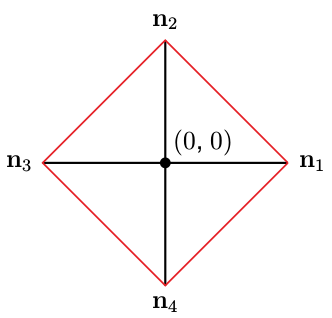
\includegraphics{imagenes/7-tensegril/PlanarTensegrity.png}
\end{figure}

We know that in a static structure the sum of the internal forces must
be equal to \(0\), so the first thing that we have to obtain is a \(F\)
that represents the sum of the internal forces.

We will begin by importing the symbolic calculus library

\begin{Verbatim}[commandchars=\\\{\}]
    {\color{incolor}In [{\color{incolor}1}]:} \PY{k+kn}{from} \PY{n+nn}{sympy} \PY{k+kn}{import} \PY{n}{init\PYZus{}printing}\PY{p}{,} \PY{n}{var}\PY{p}{,} \PY{n}{Matrix}\PY{p}{,} \PY{n}{solve}
\end{Verbatim}

\begin{Verbatim}[commandchars=\\\{\}]
    {\color{incolor}In [{\color{incolor}2}]:} \PY{n}{init\PYZus{}printing}\PY{p}{(}\PY{p}{)}
\end{Verbatim}

And initializing the symbolic variables that represent the internal
forces on the nodes.

\begin{Verbatim}[commandchars=\\\{\}]
    {\color{incolor}In [{\color{incolor}3}]:} \PY{n}{var}\PY{p}{(}\PY{l+s}{\PYZdq{}}\PY{l+s}{lambda:3}\PY{l+s}{\PYZdq{}}\PY{p}{)}
    \PY{n}{var}\PY{p}{(}\PY{l+s}{\PYZdq{}}\PY{l+s}{gamma:5}\PY{l+s}{\PYZdq{}}\PY{p}{)}\PY{p}{;}
\end{Verbatim}

We define the vectors that describe the nodes:

\begin{Verbatim}[commandchars=\\\{\}]
    {\color{incolor}In [{\color{incolor}4}]:} \PY{n}{n1} \PY{o}{=} \PY{n}{Matrix}\PY{p}{(}\PY{p}{[}\PY{l+m+mi}{1}\PY{p}{,} \PY{l+m+mi}{0}\PY{p}{]}\PY{p}{)}
    \PY{n}{n2} \PY{o}{=} \PY{n}{Matrix}\PY{p}{(}\PY{p}{[}\PY{l+m+mi}{0}\PY{p}{,} \PY{l+m+mi}{1}\PY{p}{]}\PY{p}{)}
    \PY{n}{n3} \PY{o}{=} \PY{n}{Matrix}\PY{p}{(}\PY{p}{[}\PY{o}{\PYZhy{}}\PY{l+m+mi}{1}\PY{p}{,} \PY{l+m+mi}{0}\PY{p}{]}\PY{p}{)}
    \PY{n}{n4} \PY{o}{=} \PY{n}{Matrix}\PY{p}{(}\PY{p}{[}\PY{l+m+mi}{0}\PY{p}{,} \PY{o}{\PYZhy{}}\PY{l+m+mi}{1}\PY{p}{]}\PY{p}{)}

    \PY{n}{N} \PY{o}{=} \PY{p}{(}\PY{p}{(}\PY{n}{n1}\PY{o}{.}\PY{n}{row\PYZus{}join}\PY{p}{(}\PY{n}{n2}\PY{p}{)}\PY{p}{)}\PY{o}{.}\PY{n}{row\PYZus{}join}\PY{p}{(}\PY{n}{n3}\PY{p}{)}\PY{p}{)}\PY{o}{.}\PY{n}{row\PYZus{}join}\PY{p}{(}\PY{n}{n4}\PY{p}{)}
    \PY{n}{N}
\end{Verbatim}
\texttt{\color{outcolor}Out[{\color{outcolor}4}]:}


\begin{equation*}
    \left[\begin{matrix}1 & 0 & -1 & 0\\0 & 1 & 0 & -1\end{matrix}\right]
\end{equation*}



So the vectors that describe the bars are:

\begin{Verbatim}[commandchars=\\\{\}]
    {\color{incolor}In [{\color{incolor}5}]:} \PY{n}{b1} \PY{o}{=} \PY{n}{n3} \PY{o}{\PYZhy{}} \PY{n}{n1}
    \PY{n}{b2} \PY{o}{=} \PY{n}{n4} \PY{o}{\PYZhy{}} \PY{n}{n2}

    \PY{n}{B} \PY{o}{=} \PY{n}{b1}\PY{o}{.}\PY{n}{row\PYZus{}join}\PY{p}{(}\PY{n}{b2}\PY{p}{)}
    \PY{n}{B}
\end{Verbatim}
\texttt{\color{outcolor}Out[{\color{outcolor}5}]:}


\begin{equation*}
    \left[\begin{matrix}-2 & 0\\0 & -2\end{matrix}\right]
\end{equation*}



And the strings are characterized by:

\begin{Verbatim}[commandchars=\\\{\}]
    {\color{incolor}In [{\color{incolor}6}]:} \PY{n}{s1} \PY{o}{=} \PY{n}{n2} \PY{o}{\PYZhy{}} \PY{n}{n1}
    \PY{n}{s2} \PY{o}{=} \PY{n}{n3} \PY{o}{\PYZhy{}} \PY{n}{n2}
    \PY{n}{s3} \PY{o}{=} \PY{n}{n4} \PY{o}{\PYZhy{}} \PY{n}{n3}
    \PY{n}{s4} \PY{o}{=} \PY{n}{n1} \PY{o}{\PYZhy{}} \PY{n}{n4}

    \PY{n}{S} \PY{o}{=} \PY{p}{(}\PY{p}{(}\PY{n}{s1}\PY{o}{.}\PY{n}{row\PYZus{}join}\PY{p}{(}\PY{n}{s2}\PY{p}{)}\PY{p}{)}\PY{o}{.}\PY{n}{row\PYZus{}join}\PY{p}{(}\PY{n}{s3}\PY{p}{)}\PY{p}{)}\PY{o}{.}\PY{n}{row\PYZus{}join}\PY{p}{(}\PY{n}{s4}\PY{p}{)}
    \PY{n}{S}
\end{Verbatim}
\texttt{\color{outcolor}Out[{\color{outcolor}6}]:}


\begin{equation*}
    \left[\begin{matrix}-1 & -1 & 1 & 1\\1 & -1 & -1 & 1\end{matrix}\right]
\end{equation*}



Before defining the conectivity matrix, we begin by defining \(n\)
vectors \(e_i\) with dimension \(n\), where \(n\) is the number of nodes
in the structure, and the element \(i\) in the vector is \(1\) while the
rest are all \(0\)'s.

\begin{Verbatim}[commandchars=\\\{\}]
    {\color{incolor}In [{\color{incolor}7}]:} \PY{n}{e1} \PY{o}{=} \PY{n}{Matrix}\PY{p}{(}\PY{p}{[}\PY{l+m+mi}{1}\PY{p}{,} \PY{l+m+mi}{0}\PY{p}{,} \PY{l+m+mi}{0}\PY{p}{,} \PY{l+m+mi}{0}\PY{p}{]}\PY{p}{)}
    \PY{n}{e2} \PY{o}{=} \PY{n}{Matrix}\PY{p}{(}\PY{p}{[}\PY{l+m+mi}{0}\PY{p}{,} \PY{l+m+mi}{1}\PY{p}{,} \PY{l+m+mi}{0}\PY{p}{,} \PY{l+m+mi}{0}\PY{p}{]}\PY{p}{)}
    \PY{n}{e3} \PY{o}{=} \PY{n}{Matrix}\PY{p}{(}\PY{p}{[}\PY{l+m+mi}{0}\PY{p}{,} \PY{l+m+mi}{0}\PY{p}{,} \PY{l+m+mi}{1}\PY{p}{,} \PY{l+m+mi}{0}\PY{p}{]}\PY{p}{)}
    \PY{n}{e4} \PY{o}{=} \PY{n}{Matrix}\PY{p}{(}\PY{p}{[}\PY{l+m+mi}{0}\PY{p}{,} \PY{l+m+mi}{0}\PY{p}{,} \PY{l+m+mi}{0}\PY{p}{,} \PY{l+m+mi}{1}\PY{p}{]}\PY{p}{)}
\end{Verbatim}

So, by making the same operations as before, but with the vectors
\(e_i\), we'll obtain the matrix \(D\) which is the transpose of the
\(C\) matrix.

\begin{Verbatim}[commandchars=\\\{\}]
    {\color{incolor}In [{\color{incolor}8}]:} \PY{n}{d1} \PY{o}{=} \PY{n}{e3} \PY{o}{\PYZhy{}} \PY{n}{e1}
    \PY{n}{d2} \PY{o}{=} \PY{n}{e4} \PY{o}{\PYZhy{}} \PY{n}{e2}
    \PY{n}{d3} \PY{o}{=} \PY{n}{e2} \PY{o}{\PYZhy{}} \PY{n}{e1}
    \PY{n}{d4} \PY{o}{=} \PY{n}{e3} \PY{o}{\PYZhy{}} \PY{n}{e2}
    \PY{n}{d5} \PY{o}{=} \PY{n}{e4} \PY{o}{\PYZhy{}} \PY{n}{e3}
    \PY{n}{d6} \PY{o}{=} \PY{n}{e1} \PY{o}{\PYZhy{}} \PY{n}{e4}

    \PY{n}{D} \PY{o}{=} \PY{p}{(}\PY{p}{(}\PY{p}{(}\PY{n}{d1}\PY{o}{.}\PY{n}{row\PYZus{}join}\PY{p}{(}\PY{n}{d2}\PY{p}{)}\PY{p}{)}\PY{o}{.}\PY{n}{row\PYZus{}join}\PY{p}{(}\PY{n}{d3}\PY{p}{)}\PY{p}{)}\PY{o}{.}\PY{n}{row\PYZus{}join}\PY{p}{(}\PY{n}{d4}\PY{p}{)}\PY{p}{)}\PY{o}{.}\PY{n}{row\PYZus{}join}\PY{p}{(}\PY{n}{d5}\PY{p}{)}\PY{o}{.}\PY{n}{row\PYZus{}join}\PY{p}{(}\PY{n}{d6}\PY{p}{)}

    \PY{n}{C} \PY{o}{=} \PY{n}{D}\PY{o}{.}\PY{n}{T}
    \PY{n}{C}
\end{Verbatim}
\texttt{\color{outcolor}Out[{\color{outcolor}8}]:}


\begin{equation*}
    \left[\begin{matrix}-1 & 0 & 1 & 0\\0 & -1 & 0 & 1\\-1 & 1 & 0 & 0\\0 & -1 & 1 & 0\\0 & 0 & -1 & 1\\1 & 0 & 0 & -1\end{matrix}\right]
\end{equation*}



We'll define now a \(\Lambda\) diagonal matrix, being it's elements, the
internal compression forces of the structure.

\begin{Verbatim}[commandchars=\\\{\}]
    {\color{incolor}In [{\color{incolor}9}]:} \PY{n}{Lambda} \PY{o}{=} \PY{n}{Matrix}\PY{p}{(}\PY{p}{[}\PY{p}{[}\PY{n}{lambda1}\PY{p}{,} \PY{l+m+mi}{0}\PY{p}{]}\PY{p}{,} \PY{p}{[}\PY{l+m+mi}{0}\PY{p}{,} \PY{n}{lambda2}\PY{p}{]}\PY{p}{]}\PY{p}{)}
    \PY{n}{Lambda}
\end{Verbatim}
\texttt{\color{outcolor}Out[{\color{outcolor}9}]:}


\begin{equation*}
    \left[\begin{matrix}\lambda_{1} & 0\\0 & \lambda_{2}\end{matrix}\right]
\end{equation*}



\begin{Verbatim}[commandchars=\\\{\}]
    {\color{incolor}In [{\color{incolor}10}]:} \PY{o}{\PYZhy{}}\PY{n}{B}\PY{o}{*}\PY{n}{Lambda}
\end{Verbatim}
\texttt{\color{outcolor}Out[{\color{outcolor}10}]:}


\begin{equation*}
    \left[\begin{matrix}2 \lambda_{1} & 0\\0 & 2 \lambda_{2}\end{matrix}\right]
\end{equation*}



And the \(\Gamma\) diagonal matrix, with it's elements the internal
stress forces.

\begin{Verbatim}[commandchars=\\\{\}]
    {\color{incolor}In [{\color{incolor}11}]:} \PY{n}{Gamma} \PY{o}{=} \PY{n}{Matrix}\PY{p}{(}\PY{p}{[}\PY{p}{[}\PY{n}{gamma1}\PY{p}{,} \PY{l+m+mi}{0}\PY{p}{,} \PY{l+m+mi}{0}\PY{p}{,} \PY{l+m+mi}{0}\PY{p}{]}\PY{p}{,} \PY{p}{[}\PY{l+m+mi}{0}\PY{p}{,} \PY{n}{gamma2}\PY{p}{,} \PY{l+m+mi}{0}\PY{p}{,} \PY{l+m+mi}{0}\PY{p}{]}\PY{p}{,} \PY{p}{[}\PY{l+m+mi}{0}\PY{p}{,} \PY{l+m+mi}{0}\PY{p}{,} \PY{n}{gamma3}\PY{p}{,} \PY{l+m+mi}{0}\PY{p}{]}\PY{p}{,} \PY{p}{[}\PY{l+m+mi}{0}\PY{p}{,} \PY{l+m+mi}{0}\PY{p}{,} \PY{l+m+mi}{0}\PY{p}{,} \PY{n}{gamma4}\PY{p}{]}\PY{p}{]}\PY{p}{)}
    \PY{n}{Gamma}
\end{Verbatim}
\texttt{\color{outcolor}Out[{\color{outcolor}11}]:}


\begin{equation*}
    \left[\begin{matrix}\gamma_{1} & 0 & 0 & 0\\0 & \gamma_{2} & 0 & 0\\0 & 0 & \gamma_{3} & 0\\0 & 0 & 0 & \gamma_{4}\end{matrix}\right]
\end{equation*}



\begin{Verbatim}[commandchars=\\\{\}]
    {\color{incolor}In [{\color{incolor}12}]:} \PY{n}{S}\PY{o}{*}\PY{n}{Gamma}
\end{Verbatim}
\texttt{\color{outcolor}Out[{\color{outcolor}12}]:}


\begin{equation*}
    \left[\begin{matrix}- \gamma_{1} & - \gamma_{2} & \gamma_{3} & \gamma_{4}\\\gamma_{1} & - \gamma_{2} & - \gamma_{3} & \gamma_{4}\end{matrix}\right]
\end{equation*}



It's worth noting that the \(M\) matrix that contains all of the
elements of the structure, can be obtained in two ways.

\[
M = \begin{bmatrix} B & S \end{bmatrix}
\]

\[
M = N C^T
\]

\begin{Verbatim}[commandchars=\\\{\}]
    {\color{incolor}In [{\color{incolor}13}]:} \PY{n}{M} \PY{o}{=} \PY{n}{B}\PY{o}{.}\PY{n}{row\PYZus{}join}\PY{p}{(}\PY{n}{S}\PY{p}{)}
    \PY{n}{M}
\end{Verbatim}
\texttt{\color{outcolor}Out[{\color{outcolor}13}]:}


\begin{equation*}
    \left[\begin{matrix}-2 & 0 & -1 & -1 & 1 & 1\\0 & -2 & 1 & -1 & -1 & 1\end{matrix}\right]
\end{equation*}



\begin{Verbatim}[commandchars=\\\{\}]
    {\color{incolor}In [{\color{incolor}14}]:} \PY{n}{N}\PY{o}{*}\PY{n}{C}\PY{o}{.}\PY{n}{T}
\end{Verbatim}
\texttt{\color{outcolor}Out[{\color{outcolor}14}]:}


\begin{equation*}
    \left[\begin{matrix}-2 & 0 & -1 & -1 & 1 & 1\\0 & -2 & 1 & -1 & -1 & 1\end{matrix}\right]
\end{equation*}



And due to the partition of the matrix
\(M = \begin{bmatrix} B & S \end{bmatrix}\), it simplifies the math of
the matrix \(F\):

\[
F =
\begin{bmatrix}
    -B \Lambda & S \Gamma
    \end{bmatrix} C
    \]

    \begin{Verbatim}[commandchars=\\\{\}]
        {\color{incolor}In [{\color{incolor}15}]:} \PY{n}{F} \PY{o}{=} \PY{p}{(}\PY{o}{\PYZhy{}}\PY{n}{B}\PY{o}{*}\PY{n}{Lambda}\PY{p}{)}\PY{o}{.}\PY{n}{row\PYZus{}join}\PY{p}{(}\PY{n}{S}\PY{o}{*}\PY{n}{Gamma}\PY{p}{)}\PY{o}{*}\PY{n}{C}
        \PY{n}{F}
    \end{Verbatim}
    \texttt{\color{outcolor}Out[{\color{outcolor}15}]:}


    \begin{equation*}
        \left[\begin{matrix}\gamma_{1} + \gamma_{4} - 2 \lambda_{1} & - \gamma_{1} + \gamma_{2} & - \gamma_{2} - \gamma_{3} + 2 \lambda_{1} & \gamma_{3} - \gamma_{4}\\- \gamma_{1} + \gamma_{4} & \gamma_{1} + \gamma_{2} - 2 \lambda_{2} & - \gamma_{2} + \gamma_{3} & - \gamma_{3} - \gamma_{4} + 2 \lambda_{2}\end{matrix}\right]
    \end{equation*}



    So now the only thing left to assume is the fact that the sum of the
    internal forces in each node is \(0\). The next line of code, assumes
    that every entry of the matrix is equal to \(0\), so we only have to put
    tha matrix for it to yield:

    \begin{Verbatim}[commandchars=\\\{\}]
        {\color{incolor}In [{\color{incolor}16}]:} \PY{n}{solve}\PY{p}{(}\PY{n}{F}\PY{p}{)}
    \end{Verbatim}
    \texttt{\color{outcolor}Out[{\color{outcolor}16}]:}


    \begin{equation*}
        \begin{bmatrix}\begin{Bmatrix}\gamma_{1} : \lambda_{2}, & \gamma_{2} : \lambda_{2}, & \gamma_{3} : \lambda_{2}, & \gamma_{4} : \lambda_{2}, & \lambda_{1} : \lambda_{2}\end{Bmatrix}\end{bmatrix}
        \end{equation*}



        Every force must be the same.


\subsection{String Forces}
    %\input{FuerzasdeCuerda.tex}

    Forces on the rod are due to the elongation of strings and ground reactions.
    For simplicity, we assume that the strings are Hookean, and that they are firmly attached to nodes on the rods or on fixed space coordinates.
    That is, strings are linear force elements with rest length $l_i^0$ and stiffness $k_i$.
    The force vector of the $i^{th}$ string is:

    \begin{equation}
        f(n) =
        \begin{cases}
            \hfill 0    \hfill & ||s_i|| < l_1^0 \\
            \hfill \kappa_i \left( ||s_i|| - l_1^0 \right) \left( \frac{s_i}{||s_i||} \right) \hfill & ||s_i|| \ge l_1^0 \\
        \end{cases}
    \end{equation}

    where $s_i$ is a vector in the direction of the $i^{th}$ string.
    String vectors are linear functions of the nodes of the structure as we made it the last section, assembling a matrix of string vectors and nodes.

    \begin{equation}
        S = N C_S^T \quad
        S =
        \begin{pmatrix}
            s_1 & \dots & s_m
        \end{pmatrix} \in \mathbbm{R}^{3 \times m} \quad
        N =
        \begin{pmatrix}
            n_1 & \dots & n_n
        \end{pmatrix} \in \mathbbm{R}^{3 \times n}
        \end{equation}

    where the vector $n_k$ denotes the $k^{th}$ node in the structure and the string connectivity matrix $C_S \in \mathbbm{R}^{m \times n}$, it follows that:

    \begin{equation}
        T = - S \Gamma
    \end{equation}

    where we made use of the diagonal matrix $\Gamma$ which contains the force densities on its diagonal.

    \begin{equation}
        F =
        \begin{pmatrix}
            f_1 & \dots & f_n
        \end{pmatrix} = T C_S = - N C_S^T \Gamma C_S
    \end{equation}

    It follows then, that the matrix F is the matrix of nodal forces.

\subsection{Tensegrity Structures Mechanics}
    %\input{MechanicsofTensegrityStructures.tex}

\subsection{Dynamical Analysis of Tensegrity Structures}

    The dynamics of a tensegrity structure is caracterized by the following equation

    \begin{equation}
        \left( \ddot{Q} + Q \boxminus \right) M = F_Q
    \end{equation}

    where

    \begin{equation}
        Q =
        \begin{pmatrix}
            R & B
        \end{pmatrix} =
        \begin{pmatrix}
            r_1 & \dots & r_k & b_1 & \dots & b_k
        \end{pmatrix}
    \end{equation}

    \begin{equation}
        \boxminus = \text{diag}
        \begin{pmatrix}
            0 & \dots & \xi_1 & \dots & \xi_k
        \end{pmatrix}
    \end{equation}

    \begin{equation}
        M = \text{diag}
        \begin{pmatrix}
            m_1 & \dots & m_k & J_1 & \dots & J_k
        \end{pmatrix}
    \end{equation}

    for $k$ nodes, and $F_Q$ is computed with:

    \begin{equation}
        F_Q = \left( W - Q \Psi^T C_S^T \Gamma C_S \right) \Psi^T
    \end{equation}

    where $W$ is a vector with the external forces applied in each node, $C_S$ is the conectivity matrix for the strings and $\Gamma$ is a matrix with the forces densities in the strings

    So, we can see that the prerequisites to compute the equations of motion for the system are $Q$, $\Psi$, $C_S$ and $\Gamma$.
    In this expressions we can see that $\Psi$, $C_S$ and $\Gamma$ are constant parameters of the system and $Q$, which depends on the geometry of the structure, is the only variable in the equations of motion as they satnd.

    It can be shown that this expression reduces to the following

    \begin{eqnarray}
        m_i \ddot{r}_i & = & f_{r_i} \nonumber \\
        J_i \ddot{b}_i & = & P(b) f_{b_i} - J_i b_i
    \end{eqnarray}

    where $P(b) = I - b_i b_i^T$ is the projection matrix for the orientation vector $b_i$.


%------------------------------------
	\section{Conclusions}
		Taking note of the model of two bars and 6 elements we know that the equilibrium conditions are equal force densities in each string, so we can conclude that a simple way of modelling a body with axial symetry is to asume that all the bars have the same size, the mass center of the bar is located in it's geometric center and the mass distribution is uniform, the inertial reference frame is at the origin of the positions, the friction between the rod and the string is null.

Also noting that the microtubules behave basically as rods and microfilaments as strings, we can conclude that a cell can be modelled as a class 1 tensegrity without restrictions, remaining to investigate the number of rods and strings best suited for the cell.


%------------------------------------
%         Bibliography
%------------------------------------

	\begin{thebibliography}{99} % Bibliography - this is intentionally simple in this template

		\bibitem[Joono Cheong, Robert E. Skelton, Youngsu Cho]{}
		\newblock A numerical algorithm for tensegrity dynamics with non-minimal coordinates

		\bibitem[Chandana Paul, Member, IEEE, Francisco J. Valero-Cuevas, Member, IEEE, and Hod Lipson, Member, IEEE]{}
		\newblock Design and Control of Tensegrity Robots for Locomotion

		\bibitem[Javier G. Fernandez and Donald E. Ingberb]{}
		\newblock Unexpected Strength and Toughness in Chitosan-Fibroin Laminates Inspired by Insect Cuticle

		\bibitem[Donald E. Ingber, Steven R. Heidemann, Phillip Lamoureux and Robert E. Buxbaum]{}
		\newblock Design and Control of Tensegrity Robots for Locomotion
		\newblock J Appl Physiol 89:1663-1678, 2000.

		\bibitem[Tadanori Mammoto, Akiko Mammoto and Donald E. Ingber]{}
		\newblock Mechanobiology and Developmental Control

		\bibitem[Robert E. Skelton and Mauricio C. de Oliveira]{}
		\newblock Tensegrity Systems
		\newblock DOI 10.1007/978-0-387-74242-7

		\bibitem[Donald E. Ingber]{}
		\newblock Tensegrity I. Cell structure and hierarchical systems biology
		\newblock doi:10.1242/jcs.00359

		\bibitem[Donald E. Ingber]{}
		\newblock Tensegrity II. How structural networks influence cellular information processing networks
		\newblock doi:10.1242/jcs.00360

		\bibitem[W. O. Williams]{}
		\newblock A Primer on the Mechanics of Tensegrity Structures

		\bibitem[Otger Campàs 1–4,8 , Tadanori Mammoto 3 , Sean Hasso 3 , Ralph A Sperling 1,8 , Daniel O’Connell 5 , Ashley G Bischof  2,3 , Richard Maas 5 , David A Weitz 1,6 , L Mahadevan 1,2,4,6  Donald E Ingber 1–3,7]{}
		\newblock Quantifying cell-generated mechanical forces within living embryonic tissues

		\bibitem[Dipak Panigrahy a,b,c,d,1,2 , Brian T. Kalish a,e,1 , Sui Huang f,1 , Diane R. Bielenberg a,1 , Hau D. Le a,e,g,1 , Jun Yang h , Matthew L. Edin i , Craig R. Lee j , Ofra Benny a,3 , Dayna K. Mudge a,b,c,d , Catherine E. Butterfield a , Akiko Mammoto a , Tadanori Mammoto a , Bora Inceoglu h , Roger L. Jenkins k , Mary A. Simpson k , Tomoshige Akino a , Fred B. Lih i , Kenneth B. Tomer i , Donald E. Ingber a,l , Bruce D. Hammock h,2 , John R. Falck m , Vijaya L. Manthati m , Arja Kaipainen n ,Patricia A. D’Amore o , Mark Puder a,e , Darryl C. Zeldin i,2 , and Mark W. Kieran a,b,2]{}
		\newblock Epoxyeicosanoids promote organ and tissue regeneration

		\bibitem[William J. Polacheck a , Alexandra E. German b,c , Akiko Mammoto c , Donald E. Ingber c,d,e , and Roger D. Kamm a,f,1 a]{}
		\newblock Mechanotransduction of fluid stresses governs 3D cell migration

		\bibitem[Robert E. Skelton, Rajesh Adhikari, Jean-Paul Pinaud, Waileung Chan]{}
		\newblock An Introduction to the Mechanics of Tensegrity Structures

	\end{thebibliography}

%------------------------------------
%      End of document
%------------------------------------
% \end{document}
